\documentclass[a4paper,twoside]{article}
\usepackage{listings}
\usepackage{xcolor}
\usepackage{changepage}
\usepackage{graphicx}
\usepackage[hungarian]{babel}
\usepackage{amsmath} 
\usepackage{t1enc}
\usepackage{titlesec}
\title{Szakdolgozat}

\definecolor{mygreen}{RGB}{0,128,0}
\definecolor{mygray}{RGB}{204,255,153}
\definecolor{mymauve}{RGB}{204,102,0}
\definecolor{myblue}{RGB}{0,0,204}
\definecolor{mypurple}{RGB}{204,0,204}

\graphicspath{{./images}}
\author{Bozsik József}

\lstdefinestyle{javascriptStyle}{
	language=Python,  % Change this to JavaScript
	basicstyle=\ttfamily,  % Keyword style for the second keyword list
	commentstyle=\color{mygreen},
	stringstyle=\color{mymauve},
	numberstyle=\tiny\color{mygray},
	numbers=left,
	stepnumber=1,
	numbersep=10pt,
	backgroundcolor=\color{white},
	frame=single,
	rulecolor=\color{black},
	showspaces=false,
	showstringspaces=false,
	showtabs=false,
	tabsize=2,
	captionpos=b,
	frame=none,
	breaklines=true,
	morekeywords=[1]{let, const, async, var, function, return, else, for, while, section},
	keywordstyle=[1]\color{myblue}, % Use keywordstyle1 for the first set of keywords
	morekeywords=[2]{if,await,},
	keywordstyle=[2]\color{mypurple}, % Use keywordstyle2 for the second set of keywords  % Add 'await' to the morekeywords list
	escapeinside={(*@}{@*)},
	xleftmargin=0pt,
	xrightmargin=0pt,
}

\begin{document}
\maketitle
\newpage
\tableofcontents
\newpage
{
\section*{Hallgatói nyilatkozat}}
Alulírott \textit{Bozsik József}, szigorló hallgató kijelentem, hogy ezt a szakdolgozatot meg
nem engedett segítség nélkül, saját magam készítettem, csak a megadott forrásokat (szakirodalom, eszközök stb.) használtam fel. Minden olyan részt, melyet szó szerint, vagy
azonos értelemben, de átfogalmazva más forrásból átvettem, egyértelműen, a forrás megadásával megjelöltem.
Hozzájárulok, hogy a jelen munkám alapadatait (szerző(k), cím, angol és magyar
nyelvű tartalmi kivonat, készítés éve, konzulens(ek) neve) a BME VIK nyilvánosan hozzáférhető elektronikus formában, a munka teljes szövegét pedig az egyetem belső hálózatán
keresztül (vagy autentikált felhasználók számára) közzétegye. Kijelentem, hogy a benyújtott munka és annak elektronikus verziója megegyezik. Dékáni engedéllyel titkosított diplomatervek esetén a dolgozat szövege csak 3 év eltelte után válik hozzáférhetővé.
\begin{flushleft}
	Budapest, 2022. december 6.
\end{flushleft}

\newpage
\section{Összefoglaló}
A szakdolgozat témájaként egy társasjáték készítését választottam webes környezetben mivel személy szerint mindig is érdekelt a teljes web-fejlesztési folyamat, valamint egyik kedvenc időtöltéseim közé tartozik a barátokkal egy közös társasjátékozás. 
Végül egy ''ki nevet a végén'' társas fejlesztése mellett döntöttem, hiszen a szabályok nem túl bonyolultak, viszont sok lehetőség van kreatívnak lenni az implementálás során, valamint inspirálódni is lehet az eddig elkészült játékokból amik az interneten megtalálhatók.

Társasjáték lévén, a játékot több felhasználó is játszhatja egyszerre.  Az interneten rengeteg olyan web-alkalmazás van, ahol hasonló társasjátékkal
lehet játszani, viszont a belépés nehézkes, a játék kezelése bonyolult. A célom az volt, hogy
egy letisztult felületen könnyedén és egyszerűen lehessen élvezni a társasjáték adta
élvezeteket a partnereinkkel.

Ebben a dokumentumban összefoglalom, hogy hogyan implementáltam, mind a szerveroldali,
mind a kliensoldali szoftvert. Az alkalmazás készítése során rengeteg újfajta technológiát és
keretrendszert használtam, amik jól bevált eszközök a webfejlesztésben. A munkahelyem
által biztosított szervert is használtam a megvalósításához, ami a játék logikáját biztosította. A
végeredmény egy egyszerű, és könnyen kezelhető webalkalmazás lett, ami kis
továbbfejlesztéssel versenytársa lehet az interneten található játékoknak.


\newpage
\section{Abstract}
As the topic of my thesis, I chose to create a board game in a web environment. Personally, I've always been interested in the entire web development process, and one of my favorite pastimes is playing board games with friends. Ultimately, I decided to develop a "Who Laughs Last" board game because the rules are not overly complicated, offering ample room for creativity during implementation, as well as inspiration from existing online games.

Given that it's a board game, multiple users can play it simultaneously. While there are many web applications offering similar board games online, the entry process can be cumbersome, and game management can be complex. My goal was to provide a clean interface for easily enjoying the board game with partners.

In this document, I summarize how I implemented both the server-side and client-side software. Throughout the application development, I utilized various new technologies and frameworks, proven tools in web development. I also used a server provided by my workplace to support the game's logic. The end result is a simple and user-friendly web application that, with some further development, could become a competitor to existing online games.
\newpage
\section{Bevezetés}
A webfejlesztés a mindennapi internetes böngészés során használt weboldalak és
webalkalmazások létrehozásának folyamata. Amikor egy weboldalt látogatunk, például
közösségi média platformokat, online vásárlási oldalakat vagy hírportálokat, akkor a
webfejlesztés végtermékét látjuk.
A weboldalakat programozási nyelvek, keretrendszerek és eszközök kombinációjával építik
fel. A webfejlesztés két fő komponense a frontend és a backend.
A frontend az, amit egy weboldalon látunk és amivel interakcióba lépünk. Ide tartozik az
oldal tervezése, elrendezése és felhasználói felülete, valamint a felhasználói inputok
ellenőrzése is. A frontend létrehozásához a fejlesztők olyan nyelveket használnak, mint az
HTML\footnote{Hypertext Markup Language}, CSS\footnote{Cascading Style Sheets} és a JavaScript. Az
HTML strukturálja a weboldal tartalmát, a CSS pedig esztétikus megjelenést biztosít, míg a
JavaScript interaktivitást és funkcionalitást ad hozzá.
A backend felelős a weboldal háttérlogikájáért és feldolgozásáért. Feladatokat lát el, mint az
adatok tárolása és lekérdezése, felhasználói azonosítás és a szerverkommunikáció. A
fejlesztők különböző programozási nyelveket és keretrendszereket, például az én esetemben
Java Spring\cite{javaspring}-re esett a választás mivel a munkahelyemen ezt a környezetet használják a
backend létrehozásához. Emellett adatbázisokkal kommunikálnak az információ tárolásához
és lekérdezéséhez. Az én implementációmban az utóbbi nem történt meg, hiszen a
munkahelyem által biztosított szerveren tároltam az adatokat.
A webfejlesztés gyakran API\footnote{Application Programming Interface} hívásokat tartalmaz más
szerverek felé adatok lekéréséhez vagy specifikus műveletek végrehajtásához. Ezek az API
hívások lehetővé teszik a különböző rendszerek közötti kommunikációt és információcsere
zavartalan működését. Közismert hasonlat az API-ra, hogyha egy étteremben a konyha
részleg a backend, az asztalok a frontend, ahol a vendégek (felhasználók) ülnek, akkor az API
a pincér, aki kézbesíti az ételt (adatokat).
A következő fejezetekben ismertetem, hogy az alábbi technológiákat miként valósítottam
meg, és milyen keretrendszereket használtam, amik a fejlesztést, és a felhasználói élményt is
egyaránt segítik.
\newpage

\section{Feladatkiírás pontosítása és részletes elemzése}
Magát a feladatot a külső konzulensem adta meg és specifikálta, hogy mire kell, hogy képes
legyen az alkalmazás, valamint milyen technológiákat használjunk. Maga az implementációt
teljesen rám bízta, hogy milyen osztályokat valósítok meg, azokat hogyan csoportosítom és
hogy hogyan dolgoznak együtt.
A ki nevet a végén társas szabályai vannak érvényben. Tehát egy játékos bábuja csak akkor
tud belépni a táblára, ha 6-ost dob. Ha viszont 6-ost dob valaki, akkor utána még egyszer
dobhat. Ha egy bábu ugyan arra a mezőre lép, ahol már éppen áll egy bábu, akkor leüti a
pályáról. Az a játékos győz, aki leghamarabb, az összes bábuját körbeviszi a táblán.
Mivel a web alkalmazást egy munkahelyi környezetben valósítottam meg, ott már adva volt
egy szerver, ami lényegében egy adatbázis-szerverként funkcionált, valamint játék bizonyos
szintű logikája is már implementálva volt. Tehát az alkalmazás backendjének kommunikálnia
kellett ezzel a szerverrel és feldolgoznia a válaszokat. Erre RESTful API-ra kellett küldeni a
kéréseket. RESTful API egy architekturális stílus és koncepció, amely a webes szolgáltatások
tervezését és fejlesztését írja le. A REST\footnote{Representational State Transfer} alapelveit követve
a RESTful API egy szabványos módszert nyújt a kommunikációra kliensek és szerverek
között. Ezeket az adatokat felhasználva a backend tovább küldi a frontendnek, ahol ezeket
megjeleníti.
Az alkalmazás főoldalán megjelennek az eddig létrehozott táblák, valamint információk
ezekről (hány játékos lépett már be, mennyi a maximum létszám, elindult-e már a játék,
stb…). 

Egyszerre akár több játékost is beállíthatunk. Ezután elindítjuk a pályát, ami átnavigál egy
újabb oldalra, ahol a tábla van megjelenítve. Egy adott táblának 3 státusza lehet: CREATED,
STOPPED, FINISHED. A CREATED státuszban A kockadobás egy sima gomb, amit ha a
felhasználó megnyom, generál egy számot 1-től 6-ig. Ezután rákattint a bábura amit mozgatni
szeretne, és az a megfelelő mennyiséggel előre lép a táblán. Ha éppen ellenfél játékosra lép,
leüti a tábláról. Ha az összes bábu beér akkor kiírja, hogy nyert az adott játékos és maga a
tábla átvált FINISHED státuszra. 
\newpage
\section{Alkalmazás fejlesztéséhez használt technológiák}
A modern webfejlesztésben szinte elengedhetetlen különböző keretrendszerek használata,
mivel a hatékonyságban, és a szoftverminőségben is jelentősen tud segíteni a fejlesztő
számára. 
\subsection{Frontend}

\subsubsection{Javascript keretrendszer}
Mivel az alkalmazásom felépítése több nézetből is állt, érdemes volt egy olyan keretrendszert választanom, ami támogatja a komponens 
alapú megközelítést. Ezt a  Vue.js\cite{vuejs} teljesíti is, így ezt a technológiát választottam. 

 A \textbf{komponens alapú architektúra} lényege hogy már az egyszer megírt kódunkat többször, teljesen máshol is fel tudjuk használni. Például tipikus példa 
ha listázni akarunk valamiféle adatot, bizonyos formázások után. Erre létrehozhatunk egy komponenst amit többször megjelenítünk az oldalon, vagy esetleg teljesen máshol az alkalmazásunkban (\ref{komponens}).ábra. A komponensen belül írjuk meg hogy a komponens hogyan viselkedjen, függvényeket definiálhatunk bennük, eseménykezelőket hozhatunk létre, például egy gomb megnyomására mi történjen. A komponensek egymásba ágyazhatóak így jöhet létre a szülő-gyermek viszony közöttük. Az ilyen komponensek között adatokat adhatunk át, valamint informálhatják különböző események bekövetkeztéről. 

Mivel egy társasjáték egy interaktív szórakozás, a felület sokszor fog változni, felhasználói input hatására. A letisztultság érdekében érdemes több kis komponenssel dolgozni, hiszen így az összetartózó felelősségek egy helyen vannak ezáltal könnyebb őket változtatni, valamint bővíteni a kódbázist. Viszont a komponenseknek le kell tudniuk kezelni ha valamilyen input hatására, az általuk megjelenített adatok megváltoznak. Mindezt lekezelni nagyon nehéz lenne, viszont a Vue.js segít ebben. Számon tartja azokat az adatokat amiktől függnek az egyes komponensek és automatikus frissíti őket, hogyha megváltoznak. Így tehát ha megfelelően osztjuk a komponensek felelősségeit, a felület csak azon része fog frissülni aminek muszáj, ezáltal az alkalmazásunk jól fog tudni skálázódni, ha nagyobb használatban van. 

A Vue.js számos olyan direktívát rejt, ami nagyban segíti az interaktív felület fejlesztését. Nagyon sok esetben kell több, hasonló adatot megjeleníteni a UI\footnote{User Interface}-on, erre tökéletesen használható a \textit{v-for} direktíva. Ha esetleg feltételhez kötnénk egyes elemek megjelenítését, akkor a \textit{v-if} használható (\ref{v-if}).ábra. Mindkét esetben változókat is megadhatunk, amik hogyha változnak, a keretrendszer számunkra lekezeli, és frissíti a megjelenítést.  

Komponensen belül is használhatunk \textbf{reaktív adatkötést}. Itt már fejlesztőként figyelni kell, mert itt nekünk kell megadni, hogy melyik változókat akarjuk hogy frissüljenek. A \textit{ref(variable)} kulcsszóval érhetjük hogy kövesse le a változásokat. Olyan esetek is vannak, hogy egy bizonyos feltétel mellett akarunk megjeleníteni egy komponenst vagy elemet, viszont maga a feltétel elég komplex. Erre használhatjuk a \textit{computed} tulajdonságot, ami visszaad egy értéket, és leköveti, hogyha bármilyen adat megváltozik, ami a végeredmény kiszámításához kell. Figyelhetünk is változásokat a \textit{watch} függvénnyel, ami lefut hogyha az adott változó megváltozott. 

Az alkalmazáson belül a navigáció egy fontos elem volt. A felhasználó több nézeten keresztül is navigálhat, ahol a táblák vannak listázva, vagy esetleg ahol maga a játék nézet van megjelenítve. Erre tökéletes megoldást adott a \textbf{VueRouter} (\ref{vuerouter}).ábra. Ez a funkció lehetőséget ad arra hogy egyszerűen tudjunk navigálni komponensek valamint nézetek között, amik nagy gyakorisággal URL változássokkal járnak. A VueRouter sok konfigurációs lehetőséget rejt magában, például meg lehet adni hogy minden navigáció előtt miket végezzen el. 
\begin{figure}
	\caption{Board komponens listázása}
	\begin{adjustwidth}{0cm}{10cm}
		\begin{minipage}{\textwidth}
			\begin{lstlisting}[style=javascriptStyle]
				<section>
				<Board data-test="board" v-for="board in boardStore.boards" :key="board.id" :board="board" />
				</section>
			\end{lstlisting}
		\end{minipage}
	\end{adjustwidth}
	\label{komponens}
\end{figure}

\begin{figure}
	\caption{v-if direktíva használata}
	\begin{adjustwidth}{0cm}{10cm}
		\begin{minipage}{\textwidth}
			\begin{lstlisting}[style=javascriptStyle]
				<button data-test="rollButton" v-if="isItYourPlayer"/>
			\end{lstlisting}
		\end{minipage}
	\end{adjustwidth}
	\label{v-if}
\end{figure}

\begin{figure}
	\caption{VueRouter létrehozása}
	\begin{adjustwidth}{0cm}{10cm}
		\begin{minipage}{\textwidth}
			\begin{lstlisting}[style=javascriptStyle]
				const routes: RouteRecordRaw[] = [
				{
					name: 'home',
					path: '/',
					component: App,
				},
				{
					name: 'boardManagement',
					path: '/boardManagement',
					meta: {
						hideQueryParams: true
					},
					component: BoardManagement,
				},
				{
					name: 'board',
					path: '/boardManagement/board',
					component: Board,
				},
			\end{lstlisting}
		\end{minipage}
	\end{adjustwidth}
	\label{vuerouter}
\end{figure}


\subsubsection{Állapottároló}
Mivel az alkalmazásom több komponensből állt így, egy olyan felépítést kellett alkalmaznom, hogy legyen olyan része 
az alkalmazásnak ahonnan minden szükséges adatot elérek. Erre a Pinia Store \cite{pinia}-t választottam, mivel viszonylag új technológia és könnyű használni. 
A Pinia segítségével definiálhatunk tárolókat, amelyek tárolják az alkalmazásom állapotát,
és különböző metódusokat határozhat meg az állapot módosítására. Minden tároló külön
példányként jön létre, lehetővé téve az alkalmazás állapotának területenkénti vagy funkció
szerinti elválasztását és \mbox{szervezését}. Ezt én két kategóriába soroltam: Azok az állapotok amik a táblák kezelésével foglalkoznak, például új táblák
létrehozása, vagy játékos csatlakozása a pályához, vagy a játékmenettel kapcsolatos tevékenységek mint a dobás vagy lépés a pályán (\ref{pinia}.ábra). 
A Pinia egyik fő előnye a reaktivitási rendszere. A Vue reaktivitását használja fel, hogy
automatikusan frissítse a komponenseket, amikor az állapot a tárolóban megváltozik. Ez
biztosítja, hogy az alkalmazásom mindig szinkronban legyen, és lehetővé teszi a
felhasználói felület hatékonyabb megjelenítését. Így tehát ha egy Pinia Store-beli állapotra hivatkozom a komponensemben, az ugyanúgy reaktív fog maradni a változás után is. 

\begin{figure}
	\caption{GamePlay store definiálása állapotokkal és függvényekkel}
	\begin{adjustwidth}{0cm}{10cm}
		\begin{minipage}{\textwidth}
			\begin{lstlisting}[style=javascriptStyle]
				export const useGamePlayStore = defineStore('gamePlayStore', {
					
					state: () => {
						return {
							rollResponse: {}, errorOccured: false, errorMessage: "", thrownNumber: 0,
							currentPlayer: {}, disableRollButton: false, players: [], playingBoard: {},
							selectedPiece: {}, robotEnabled: false, robotStrategy: null
						}
						
					},
					
					actions: {
						async rollDice(boardId, playerId) {
							try {
								this.rollResponse = await gameplayStoreApi.rollDice(boardId, playerId);
								
							} catch (error) {
								console.log(error);
								this.errorMessage = error.response.data;
								this.errorOccured = true;
								
							}
						},
						async movePlayer(boardId, moveRequest) {
							try {
								
								const updatedBoard = await gameplayStoreApi.movePlayer(boardId, moveRequest);
								this.disableRollButton = false;
								//this.playingBoard = updatedBoard;
								if (this.playingBoard.nextPlayerId) {
									this.currentPlayer = updatedBoard.players.find(p => p.id === updatedBoard.nextPlayerId);
								}
							}
							catch (error) {
								console.log(error.response);
							}
						},
			\end{lstlisting}
		\end{minipage}
	\end{adjustwidth}
	\label{pinia}
\end{figure}
\subsubsection{Modul csomagoló}

A Webpack\cite{webpack} egy népszerű modulbundler JavaScript alkalmazásokhoz. Gyakran
használják webfejlesztésben ahhoz, hogy egy alkalmazás különböző moduljait,
erőforrásait és függőségeit egyetlen fájlba vagy fájlcsoportba csomagolja. A Webpack fő
célja a teljesítmény optimalizálása és a modern webalkalmazások bonyolultságának
kezelése.

A Webpack moduláris megközelítést alkalmaz, amely lehetővé teszi a fejlesztők számára,
hogy a kódbázist külön modulokra bontsák. Elemzi ezeknek a moduloknak a függőségeit
és létrehoz egy függőségi gráfot. Ezen gráf alapján a Webpack összecsomagolja a
modulokat, feloldja a függőségeket és generálja a végső kimeneti fájlokat.

\subsubsection{HTTP kérések küldése}
A webalkalmazások felépítésé egyszerűen megfogalmazva a következő: A backend-ről szolgáltatjuk az adatokat ahova a kliens alkalmazás, más szóval a frontend kéréseket küld. Ezeket a kéréseket HTTP kérésekként küldi el az interneten keresztül. Ez az egyik legfontosabb feladat funkcionális téren. Mivel ilyen esszenciális 
ezt megvalósítani, ezért segédkönyvtárat használtam fel a könnyebb és jobb megvalósítás érdekében. Az Axios\cite{axios} könyvtárat használtam fel, mivel az egyik legnépszerűbb, így remek dokumentáció tartozik hozzá, és egyszerű a szintaxisa. 

Jól strukturált API-t biztosít a HTTP kérések kezeléséhez.Különböző HTTP metódusokat, például GET, POST,
PUT, DELETE stb. használhatunk a kérések elküldésére (\ref{axios}).ábra. Ezek a kérések szinte folyamatosan zajlanak a játék során, így fontos hogy ne legyenek zavaróak és hogy ne akadjon meg emiatt az alkalmazás, hiszen ez nagyban rontaná a felhasználói élményt. Az \textbf{Axios aszinkron kérések} kezelésére épül, amely
lehetővé teszi az alkalmazás folyamatosságát és reaktivitását. Nem blokkolja a fő
szálat, így más műveletek végrehajtására is lehetőséget ad, tehát a felület ugyanúgy működik, nem lesz észrevehető "befagyás".
További előnye a könyvtárnak, a konfigurálhatósága az Axios példánynak. Meg tudjuk adni, hogy minden egyes kéréssel együtt például egy bizonyos fejlécet csatoljon, vagy esetleg minden válasznál ellenőrizze a státuszt. Ez nagyban megkönnyíti a kódolást, valamint a hibázástól is óv, hiszen csak egyszer kell jól megírni a használni kívánt példányt. 
\begin{figure}
	\caption{Post HTTP kérés Axios könyvtárral}
	\begin{adjustwidth}{0cm}{10cm}
		\begin{minipage}{\textwidth}
			\begin{lstlisting}[style=javascriptStyle]
					this.authTokens = (await axios.post("http://localhost:8080/auth/createToken", {authCode: code})).data
					\end{lstlisting}
				\end{minipage}
	\end{adjustwidth}
\label{axios}
\end{figure}

\subsubsection{Grafikus könyvtár}
Természetesen maga a pályát meg kellett tudnom rajzolni. Mivel egész alkalmazásomnak ez a lényege, így természetesen egy külső könyvtárat használtam, hogy minél egyszerűbben és minél szebben tudjam éltre kelteni a társasjátékot. Ehhez a Konva könyvtárat választottam, mert kiemelkedően jó dokumentáció tartozott hozzá, és mivel előtte még nem foglalkoztam ilyen grafikus könyvtárakkal fontos volt hogy könnyedén meg tudjam tanulni. Valamint egyszerű, de mégis sokféle funkcióval rendelkezik amiket felhasználhattam a fejlesztés során. 
Ez a könyvtár lehetővé teszi a fejlesztők számára, hogy könnyedén rajzolhassanak formákat, vonalakat, szövegeket és egyéb grafikai elemeket a webes felületeken, és interaktív alkalmazásokat hozzanak létre, ahol a felhasználók rajzolhatnak, mozgathatnak és manipulálhatnak grafikai elemeket.Az alábbiakban néhány kulcsfontosságú tulajdonság és funkció, amelyeket a Konva nyújt:
\begin{itemize}
	\item \textbf{HTML5 Canvas alapú:} Konva a HTML5 Canvas API-t használja, ami lehetővé teszi a közvetlen grafikus rajzolást a webes felületeken. Ez rendkívül hatékony és lehetővé teszi a komplex grafikai elemek létrehozását.
	\item \textbf{Interaktivitás:} Konva lehetővé teszi az interaktív grafikus elemek létrehozását, például húzható és áthelyezhető elemeket, melyekre kattintva változtathatjuk az állapotukat.
	\item \textbf{Rétegek és Csoportok:} A könyvtár támogatja a rajzok elrendezéséhez használt rétegek és csoportok létrehozását, ami rendszerezheti és kezelheti a grafikai elemeket.
	\item \textbf{Szöveg és betűtípusok:} Konva lehetővé teszi a szöveges elemek létrehozását, és támogatja a különböző betűtípusok és formázási lehetőségek használatát.
	\item \textbf{Animáció:} A könyvtár animációt támogat, így a grafikai elemek mozgathatók és animálhatók.
	\item \textbf{Eseménykezelés:} Konva lehetővé teszi az események kezelését, például kattintásokat és húzásokat, ami lehetővé teszi az interaktív műveletek megvalósítását (\ref{konva}.ábra)
	\item \textbf{Több platform támogatása:} A Konva nem csak böngészőkben használható, hanem akár Node.js környezetben is, ami különféle alkalmazások fejlesztését teszi lehetővé.
\end{itemize}

\begin{figure}
	\caption{Kör létrehozása és eseménykezelő aktiválása Konva-val}
	\begin{adjustwidth}{0cm}{10cm}
		\begin{minipage}{\textwidth}
			\begin{lstlisting}[style=javascriptStyle]
				var circle = new Konva.Circle({
					x: currentX,
					y: currentY,
					radius: 500 / numberOfFields,
					fill: 'white',
					id: id.toString(),
					stroke: 'black',
					strokeWidth: 1
				});
				(function (caputerCircle) {
					caputerCircle.on("mousedown", function () {
						const piece = gamePlayStore.currentPlayer.pieces.find(p => p.positionOnTheBoard == caputerCircle.id());
						if (piece) gamePlayStore.selectedPiece = piece;
						
					});
				})(circle);
				
			\end{lstlisting}
		\end{minipage}
	\end{adjustwidth}
	\label{konva}
\end{figure} 

\subsection{Backend}

\subsubsection{Java keretrendszer}
A backend részt JavaSpringben\cite{javaspring} valósítottam meg. A Spring lehetővé teszi a gyors és hatékony
webalkalmazások építését, miközben egy rugalmas és moduláris környezetet biztosít a
fejlesztőknek.
\begin{itemize}
	\item  \textbf{Inversion of Control - IoC:} A Spring keretrendszer alapvetően az IoC elvet követi,
	amelyben a keretrendszer vállalja a felelősséget az objektumok létrehozásáért,
	konfigurálásáért és összekapcsolásáért. Ez lehetővé teszi a komponensek laza
	összekapcsolását és könnyen cserélhetővé teszi az implementációkat.
	\item \textbf{Dependency Injection - DI:} A Spring keretrendszer segítségével a dependency
	injection könnyen megvalósítható. Ez azt jelenti, hogy a szükséges objektumokat egy
	külső forrásból szúrhatjuk be a komponensekbe anélkül, hogy a komponenseknek
	maguknak kellene létrehozniuk vagy tudniuk kellene róluk. Ez elősegíti a lazán
	összekapcsolt és könnyen karbantartható kód írását.
	\item \textbf{Webalkalmazás támogatás:} A Spring keretrendszer számos modult és komponenst
	kínál a webalkalmazások fejlesztéséhez. A Spring MVC (Model-View-Controller)
	modell segítségével könnyedén készíthetünk hatékony és rugalmas webes
	alkalmazásokat. A Spring Boot pedig egy továbbfejlesztett modul, amely lehetővé
	teszi a gyors és egyszerű konfigurációt és a gyors indítást.Több előnye is van a Spring
	keretrendszernek, viszont mivel az alkalmazásom bonyolultsága nem követelte meg a
	használatukat, így ezeket nem részletezném.
\end{itemize}

\subsubsection{Lombok}
Egy Model osztály esetében rengetegszer fordul elő, hogy ugyanazt a kódot kell megírni, nagyon kicsit változtatásokkal minden osztály esetében. Ezt nevezzük boilerplate kódnak, ami olyan alapvető vagy sablonkód, amely gyakran ismétlődő és rutinszerű feladatokra szolgál. Mivel ez renget időt emészt fel, így ezt a problémát egy könyvtár segítségére bíztam. 
A Lombok \cite{lombok}  egy Java nyelvű könyvtár, amely
segít csökkenteni a boilerplate kódot és növeli a fejlesztési produktivitást.  A Lombok annotációkat használva (\ref{lombok}.ábra) lehetővé teszi, hogy a fejlesztők egyszerűbben és gyorsabban hozzanak létre Java osztályokat. Annotációkat a programozásban gyakran használnak, mivel segítik a kód megértését, segíthetik a fejlesztőt a kódírás minimalizálásában, vagy akár a dokumentáció írásában. A Java nyelvben többféle annotációk léteznek. Ilyenek például a beépített annotációk, amik segítik a kód
megértését. A @Deprecated annotációval ellátott elemeket jelölik, hogy elavultak vagy nem ajánlottak használatra. Ez figyelmezteti a fejlesztőket, hogy más megoldást vagy alternatívát kell használni.

\begin{figure}[h]
	\caption{Lombok annotációk használata}
	\centering
	\begin{lstlisting}[language=java]
		
	@Data
	@NoArgsConstructor
	@AllArgsConstructor
	public class MoveRequestDTO {
		
		private String pieceId;
		private String playerId;
		
		private String token;
	}
		
	\end{lstlisting}
	\label{lombok}
\end{figure} 

\subsubsection{Autentikációs keretrendszer}
Az autentikációhoz egy Third Party Software-t akartam Használni. Ez azt jelenti, hogy hasonlóan mint a könyváraknál, már előre megírt szoftvert fogok használni. Arra volt szükségem, hogy egyszerűen meg tudjam adni a belépési beállításokat, valamint hogy szerepekhez tudjam rendelni a bejelentkezett felhasználókat, hiszen nem biztos, hogy mindenki ugyanazzal a jogosultságokkal rendelkezik. Ezekkel a kritériumokkal a Keycloak\cite{keycloak} keretrendszer tűnt az ideális választásnak. 

A Keycloak egy sor olyan funkciót kínál, amelyek segítenek az alkalmazások és szolgáltatások biztonságosításában, ideértve a Single Sign-On (SSO), felhasználói hitelesítést, felhasználói engedélyezéseket és az azonosítás közvetítését. A Single Sign-On (SSO) egy olyan hitelesítési és azonosítási technológia, amely lehetővé teszi a felhasználók számára, hogy egyszeri bejelentkezéssel hozzáférjenek több különböző alkalmazáshoz vagy rendszerhez anélkül, hogy minden egyes alkalmazásban külön-külön be kellene jelentkezniük. Ennek előnyei közé tartozik a a felhasználói kényelem, szigorú ellenőrzés, könnyebb felhasználói ellenőrzés. A Keycloak olyan megoldást nyújt, amely egyszerűsíti a biztonság hozzáadásának folyamatát az alkalmazásokhoz, és lehetővé teszi a felhasználói azonosításokat, szerepeket és jogosultságokat központilag történő kezelését (\ref{keycloak-login}.ábra). A keretrendszert integrálni lehet különböző alkalmazásokkal és platformokkal, így értékes eszköz azoknak a szervezeteknek, akik webalkalmazásaikat és API-ikat szeretnék biztonságossá tenni. Ezt felhasználva tudtam a backendről http kéréseket végezni a szintén lokálisan futó Keycloaknak, hogy autentikálja a belépett felhasználót. Támogat különböző hitelesítési módszereket, beleértve a közösségi bejelentkezéseket, több tényezős hitelesítést és még sok mást. Emellett a Keycloak rendkívül rugalmas és bővíthető architektúrával rendelkezik, így alkalmas különféle felhasználási esetekre, a kis alkalmazásoktól a nagyvállalati rendszerekig. Gazdag API-kat kínál, és egy felhasználóbarát adminisztrációs konzolt, amely segít a felhasználók, valóságok és ügyfelek kezelésében.

\begin{figure}
	\caption{Keycloak konfigurációs nézete}
	\raggedleft 
	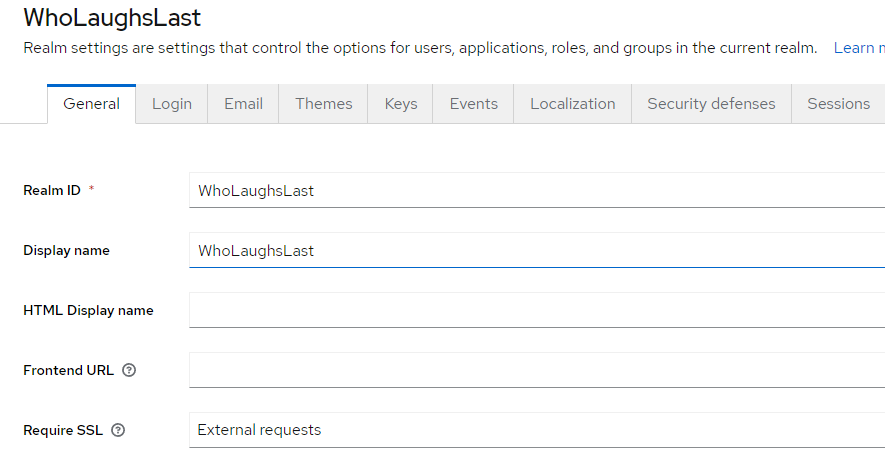
\includegraphics[scale=0.5]{keycloak-login}
	\label{keycloak-login}
\end{figure}

\subsubsection{Többjátékos mód megvalósítása}
Mivel a társasjáték csak akkor tud működni ha legalább ketten játszanak vele, így implementálnom kellett olyan funkciókat amik lehetővé teszik, hogy értesüljenek 
a felhasználók egymás lépéseiről. Mivel a kliens alkalmazás minden felhasználó gépén külön fut, így természetes, hogy a backenden kell ezt a funkciót megvalósítani, hiszen ez az egyetlen közös pont a játékosoknál. Ennek a funciónak a megvalósításához két féle ötlet létezik. A Server-Sent-Events (SSE) vagy a Websocket. Mindkettő olyan technológiák, amelyek lehetővé teszik a kliens és a szerver közötti valós idejű kommunikációt a weben keresztül, de különböznek a működésük és a használatuk szempontjából. Websocket esetében kétirányú kommunikációt tesz lehetővé, ami azt jelenti, hogy mind a kliens, mind a szerver küldhet üzeneteket egymásnak bármikor. A kapcsolat felépítéséhez WebSocket protokollt használja, ami később egy WebSocket kapcsolathoz vezet. Az SSE esetében egyirányú kommunikációt biztosít a szerverről a kliens felé. Csak a szerver küldhet adatokat a kliensnek. Az SSE beépített támogatást nyújt az automatikus újraépítéshez, ami azt jelenti, hogy ha a kapcsolat megszakad, a böngésző automatikusan megpróbálja újraépíteni. Könnyen használható és könnyen implementálható a böngészőben, és a szerveroldalon is könnyen konfigurálható. Mivel az én esetemben csak a klienst kellett értesíteni, hogy a játék állása, státusza megváltozott így a SSE technológiát választottam (\ref{sse}.ábra). 
\begin{figure}[h]
	\caption{SSE szerver osztály annotációi}
	\centering
	\begin{lstlisting}[language=java]
		
	@RestController
	@CrossOrigin(origins = "http://localhost:3000")
	@Component
	public class EventSender {
		
		public List<SseEmitter> emmitters = new CopyOnWriteArrayList<SseEmitter>();
		
	\end{lstlisting}
	\label{sse}
\end{figure} 
\subsubsection{Tesztelés}
A backend API teszteléséhez, frontend nélkül, kiváló megoldást kínál a Postman\cite{postman}, így ezt használtam a fejlesztés során. Az alábbiakban néhány kulcsfontosságú jellemzőt és funkciót ismertetek, amit a Postman kínál:

\begin{itemize}
	\item \textbf{API Tesztelés:} Postman segítségével könnyedén készíthetsz és futtathatsz API-teszteket. Különböző HTTP kéréseket küldhetsz az API-hoz, és az eredményeket vizsgálhatod.
	\item \textbf{Környezetek és Változók:} Lehetőséged van környezeteket és változókat definiálni a kérésekben, ami lehetővé teszi különböző környezetek (pl. fejlesztési, tesztelési, élő) közötti könnyű váltást és paraméterezést.
	\item \textbf{Automatizálás:} Postman segítségével automatizálhatod az API-teszteket és kéréseket. Például létrehozhatsz kollekciókat, amelyeket később futtatni tudsz automatizált módon.
	\item \textbf{Hitelesítés és Biztonság:} A Postman lehetővé teszi különböző hitelesítési mechanizmusok, például API kulcsok vagy OAuth használatát. Emellett támogatja a biztonsági teszteket is.
\end{itemize}




\newpage



\section{Önálló munka bemutatása}
Első részben az alkalmazás backendjét írtam meg, mert felépítésben így tűnt
logikusnak. Az osztályokat rétegekbe rendeztem funkciójuk és függőségeik szerint.
\subsection{Backend}
A backend részét a Java Spring projektben valósítottam meg. Ehhez a Spring Initializr-t használtam, mivel meggyorsítja a projekt létrehozásának a feladatát. Itt
egyszerűen meg lehet adni, hogy milyen függőségeket szeretnénk használni a projektünk során, majd ezután egy zip fájlként le is tölthetjük a gépünkre. Ebben a projektben már be lesznek téve azok az xml tag-ek a pom.xml fájlba, amik leírják a függőségeinket. Ehhez természetesen a fejlesztés során is rakhatunk hozzá. 
A Model rétegbe tettem azokat az osztályokat, amiket majd, később a hálózaton elküldök egy
http (HyperText Transfer Protocol) kérésbe ágyazva a szervernek, majd a válaszokat is ezekbe
az osztályokba konvertálom át. Az egész backenden ezekkel az objektumokkal dolgozok.
A DAL (Data Acces Layer)-be tettem azokat az osztályokat amik kommunikálnak a
szerverrel. Esetünkben a nevezéktan egy kicsit megtévesztő, hiszen hagyományos web
alkalmazás esetén ez a réteg az adatbázissal kommunikál, ám ennek hiányában nekünk erre
nincs lehetőségünk. Az elnevezést viszont megtartottam, hiszen gondolhatunk a szerverünkre,
mint egy okos adatbázisra, ami ismeri a ki nevet a végén társas szabályait, valamint, ha egy
másik fejlesztő olvasná a kódomat, egyből tudná, hogy az adott rétegnek mi a felelőssége.
Ezekben az osztályokban indítom el a http kéréseket, valamint a válaszokat is itt konvertálom
vissza DTO (Data Transfer Object)-re és adom tovább a BLL (Buisness Logic Layer)
rétegnek.
A BLL rétegnek különösebb jelentősége nincs. Megvalósítottam viszont, hiszen sosem lehet
tudni, hogy mikor kell továbbfejleszteni, egy új funkcióval bővíteni az alkalmazást, aminek a
logikájának a megírását ebben a rétegben kell implementálni. Hagyományos esetben itt
végeznénk el az adatok esetleges transzformációját, az üzleti logikánk itt valósulna meg. Az
én esetemben viszont erre nincsen szükség hiszen már a konzisztens adatot (vagy esetleges
hibaüzenetet) kapom vissza, közvetetten a szervertől, így itt csak egy továbbhívás történik a
DAL réteg felé.
A Controller rétegben definiálom azokat az API végpontokat, amiket majd a később megírt
frontendem fog hívni. Ez a réteg indítja el a kérések sorozatát, ami végigfut a backenden,
majd visszatér a szervertől kapott adattal (\ref{backend-pipeline}. ábra).

Ahogy már korábban említettem, a munkahely által biztosított szerverre kellett http kéréseket
küldeni. Ehhez volt egy Swagger\cite{swagger} oldal, hogy milyen API végpontok vannak a szerveren, és
azokhoz milyen URL tartozik.  Az is le volt írva, hogy milyen DTO-kat kell definiálni a
kommunikációhoz. Ezért így először létrejött a DTO, avagy Model mappa, ahol deklaráltam a
megfelelő osztályokat. A dokumentációban részletezve volt, hogy bizonyos híváshoz milyen
paramétert kell átadni, valamint mit fog visszaadni. Például, ha egy új táblát szeretnék
felvenni, akkor az adott POST kérésnél milyen DTO-t kell elküldeni, és milyen objektumot
fog visszaküldeni. Ez általában a http kérés body-jában küldték, onnan kellett kikonvertálni. Szerencsére ez Spring keretrendszernek hála, nagyon könnyen meg tudtam csinálni (\ref{post-vegpont}.ábra).
\begin{figure}[h]
	\caption{Egy post végpont a backenden}
	\raggedleft
\begin{adjustwidth}{0cm}{10cm}
	\begin{minipage}{\textwidth}
	\begin{lstlisting}[language=java]
		
@PostMapping("/board")
public ResponseEntity<?> createBoard(@RequestBody CreateBoardDTO board) {
	BoardDTO createdBoard = null;
	try {
		createdBoard= boardService.createBoard(board);
		
	}catch (ErrorCodeException e) {
		return new ResponseEntity<>(e.getErrorCode().
		getErrorCode(),HttpStatusCode.valueOf(400));
	}
	catch(Exception e){
		System.out.println(e);
	}
	return new ResponseEntity<>(createdBoard,HttpStatusCode
	.valueOf(200));
}
	\end{lstlisting}
\end{minipage}
\end{adjustwidth}
	\label{post-vegpont}
\end{figure} 

Magán a szerveren a játék logikája már implementálva volt, így mindig
konzisztens adatokat kaptunk vissza, tehát például egy táblán nem lehet két ugyanolyan nevű
játékos. Ha esetleg egy ilyen kérés érkezett akkor egy ErrorMessage osztállyal tért vissza,
amiben részletezve volt a hiba.

\begin{figure}
	\caption{Egy kérés kiszolgálásának folyamata}
	\raggedleft 
	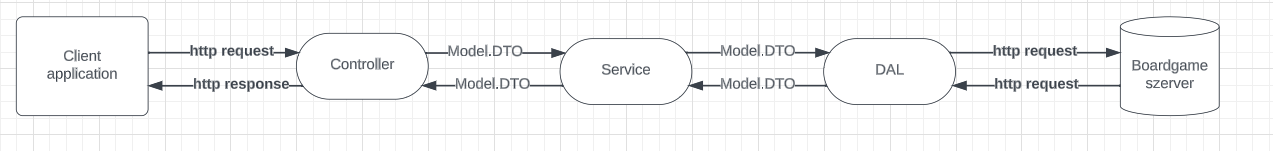
\includegraphics[scale=0.5]{backend-pipeline}
	\label{backend-pipeline}
\end{figure}

Az implementáció után a kód tesztelése volt hátra, mivel az iparban elvárt a tesztesetek írása hiszen számos előnnyel jár.
Egységtesztelést végeztem, ami azt jelenti hogy mindig csak egy alap funkciót teszteltem le, ez általában egy osztály és annak függvényei. Többféle tesztelés is létezik, például integration test, ami az egységek együttműködését teszteli, valamint end-to-end tesztek amik az egész alkalmazást fedik le. Az a jó hogyha lefelé haladva ezen a tesztelési hierarchián, egyre több tesztünk van. Egységtesztelés 
alatt a fejlesztők sok mindenre rájöhetnek a kódbázissal kapcsolatban. Például hogy a felelősségeik hogyan vannak elosztva. Ha egy osztályt nehéz tesztelni, az valószínűleg azért van, mert nagyban függ más komponensektől. Ez egy jele annak hogy rossz a design a kódban, hiszen hogyha egy osztály nagyban függ más osztályoktól, akkor ha azok megváltoznak, az erre is hatással lesz így a fenntarthatóság jóval nehezebb lesz. A tervezésnél fontos hogy lazán csatoltak legyenek az osztályok, hogy ilyen ne fordulhasson elő. Másik fontos előnye a tesztek írásának, hogy amikor újraírunk egy kódrészletet, esetleg optimálisabbá akarjuk tenni, akkor a tesztek segítségével ellenőrizhetjük, hogy megmaradt-e a kívánt funkcionalitás.  Mivel rétegeltem, a különböző funkciókat így könnyedén tudtam tesztelni őket, hiszen
egy mockolás (a Mockito [7] könyvtárat használtam ehhez) után egyszerűen tudtam tesztelni (\ref{mocking}.ábra).
A "mockolás" egy olyan technika, amelyben a tesztelés során a valódi rendszerek vagy
komponensek helyett szimulált, viselkedést utánzó objektumokat (mock objektumokat) használnak.
A mock objektumok olyan mesterségesen létrehozott objektumok, amelyek az
eredeti rendszer vagy komponens egy részét helyettesítik, és előre definiált válaszokat adnak a
függvényhívásokra vagy metódusokra. A mock objektumok segítségével szimulálhatók a
valós környezetben előforduló esetek, például adatbázishoz való kapcsolódás vagy hálózati
kommunikáció, anélkül hogy a valódi rendszerre vagy szolgáltatásra támaszkodnánk. Ez a technika jó design esetén is szükséges hiszen, nem lehet teljesen független modulokból egy működő alkalmazást csinálni, valamiféle együttműködés feltétlen szükséges. 
\begin{figure}[h]
	\caption{Függőségek mockolása a tesztben}
	\raggedleft
	\begin{lstlisting}[language=java]
		
	public class GamePlayDAOTest {
		
		GamePlayDAO gamePlayDAO;
		
		HttpClientFactory httpClientFactory;
		
		HttpClient client;
		HttpResponse response;
		
		@BeforeEach
		void mocking () throws Exception{
			httpClientFactory = mock(HttpClientFactory.class);
			client = mock(HttpClient.class);
			response = mock(HttpResponse.class);
			gamePlayDAO = new GamePlayDAO(httpClientFactory);
			when(httpClientFactory.getNewHttpClient())
			.thenReturn(client);
			when(client.send(any(),any())).thenReturn(response);
		}
	\end{lstlisting}
	\label{mocking}
\end{figure} 
Ahhoz hogy többjátékos módot támogassa a backend, a Server-Sent-Events technológiát alkalmaztam és implementáltam le. Itt a munkahelyi szerveren létre volt hozva egy interfész,WhoLaughslastMessagingProcessor néven, amit implementálni kellett (\ref{messproc}.ábra). Alapvetően 4 darab eseményről értesítjük az összes felhasználót: \begin{enumerate}
	\item Felhasználó dobott a kockával.
	\item Felhasználó lépett egy bábuval.
	\item Játékos csatlakozott egy táblához.
	\item A játék státusza megváltozott (Például egy játékot elindítottak akkor CREATED státuszról STARTED státuszra vált).
\end{enumerate}
Az első esetben az adat amit küldünk a kliens alkalmazásnak az új pálya helyzetét leíró adatok. Tehát hogyha egy játékos lépett akkor a bábu helyzete, a visszaküldött JSON válaszban már az újat reprezentálja. A második esetben megkapjuk, hogy hányast dobott az adott játékos, valamint ki a soron következő játékos. A 3. és a 4. esetben az új táblát leíró JSON adatot küldi el. Azok az osztályok amiket itt elküld, azok a munkahelyi szerverről származnak, ott hívják meg őket a megfelelő objektumokkal. Viszont mivel a frontendről kialakítottuk a kapcsolatot, ezeket az eseményeket mind megkapja az alkalmazás. Viszont ilyen esetben egy olyan probléma merül fel, mivel egyszerre akár többen is használhatják az alkalmazást, tehát nem biztos hogy csak 1 tábla van használatban akár lehet több is. Hiszen tegyük fel egyszerre 2 társaság dönt úgy, hogy játszik az alkalmazással, akkor azokat az eseményeket amik az ő táblájukon történik, másik társaság kliens alkalmazása is megkap. Ez természetesen megengedhetetlen, hiszen ha az egyik társaság befejezi a játékot és a táblájuk a FINISHED státuszra vált, akkor a másik társaság játéka is befejeződne, akár kész vannak, akár nem. Tehát meg kell valahogy különböztetni a küldött eseményeket, mégpedig táblánként, hogy az adott eseményekre való feliratkozásnál csak azokra figyeljen, ami a releváns pályán történik. Eseményt az \textit{EventSender} osztály \textit{send} metódusával lehetséges. Itt megadhatunk paraméterben egy szöveget, ami az eseménynek a neve lesz, amire később referálhatunk a frontenden, hogy melyik eseményre akarunk hivatkozni. Itt paraméterben adtam meg a táblának az \textit{id} tulajdonságát, ami minden táblánál egyedi. Így biztosítani tudtam, hogy a feliratkozásnál, csak a releváns táblára iratkozik fel, így nem lesz probléma egyidejű játéknál több felhasználónál. 
\begin{figure}[h]
	\caption{WhoLaughslastMessagingProcessor interfész implementálása}
	\raggedleft
	\begin{lstlisting}[language=java]	
@Component
@RequiredArgsConstructor(onConstructor = @__(@Autowired))
public class MessagingProcessor implements WhoLaughLastMessagingProcessor{
	private final EventSender sender;
	@Override
	public void playerUpdated(PlayerUpdateMessage playerUpdateMessage) {
		System.out.println("PlayerChange"+playerUpdateMessage
		.getBoardId());
		sender.sendEvents("PlayerChange"+playerUpdateMessage
		.getBoardId(),playerUpdateMessage);
	}
	@Override
	public void rolledDice(RolledDiceMessage rolledDiceMessage) {
		sender.sendEvents("RollChange"+rolledDiceMessage
		.getBoardId(),rolledDiceMessage);
	}
	@Override
	public void move(PositionsUpdateMessage positionsUpdateMessage) {
		
		sender.sendEvents("PositionChange"+positionsUpdateMessage
		.getBoardId(),positionsUpdateMessage);
	}
	@Override
	public void gameStatusChange(BoardStatusChangeMessage
					 boardStatusChangeMessage) {
		sender.sendEvents("StatusChange"+boardStatusChangeMessage
		.getBoardId(),boardStatusChangeMessage);
	}
}
		\end{lstlisting}
		\label{messproc}
	\end{figure} 
Valamint még szükség volt arra az osztályra (\ref{eventsender}.ábra) ami magát az eseményeket elküldi a kliens számára.  Egy \textit{SseEmitter} osztályú objektumokból álló listát is létrehoztam mint tagváltozó, itt tárolom a különböző klienseknek a feliratkozását. Ez nagyon fontos hogy CopyOnWriteArrayList típusú legyen, mivel így kezelhető a konkurencia.Valamint létrehoztam egy újabb végpontot, amit majd az \textit{EventSource} létrehozásánál hivatkozhat a frontend.  Ha ez a hívás megtörténik, akkor először létrehozok egy emittert, aminek konstruktorában a \textit{\texttt{LONG.MAX\_VALUE}} értéket adom. Ez az érték azt jelenti hogy egyes emitterek mennyi ideig tartsák fent a kapcsolatot mielőtt megszakítják a kapcsolatot. Ezek után létrehozok egy \textit{SseEmitter} osztályú objektumot ami küld egy \textbf{"INIT"} nevű eseményt, majd ezt az emittert az osztály tagváltozójához hozzáadom. Deklaráltam egy függvényt \textit{sendEvents} néven, ami végigiterál ezeken az emitter-eken, és elküldi a paraméterben átadott névvel és adattal, az eseményt a kliens alkalmazásnak.   
\begin{figure}[h]
	\caption{EventSender osztály implementálása}
	\centering
	\begin{lstlisting}[language=java]	
@RestController
@CrossOrigin(origins = "http://localhost:3000")
@Component
public class EventSender {
		
	public List<SseEmitter> emmitters = new CopyOnWriteArrayList
	<SseEmitter>();
		
	@RequestMapping("/subscribe")
	public SseEmitter subscribe() {
	System.out.println("Subscripbed");
		SseEmitter emmitter = new SseEmitter(Long.MAX_VALUE);
		try{
			emmitter.send(SseEmitter.event().name("INIT"));
		}catch (IOException e) {
			e.printStackTrace();
		}
		emmitter.onCompletion(() -> emmitters.remove(emmitter));
		emmitters.add(emmitter);
		return emmitter;
		
	}
	public void sendEvents(String eventname, Object data){
		for(SseEmitter emitter : emmitters){
			try{
				emitter.send(SseEmitter.event().name(eventname)
				.data(data));
			}catch(IOException e){
				emmitters.remove(emitter);
			}
			}
		}
	}
	\end{lstlisting}
	\label{eventsender}
\end{figure} 



\subsection{Authentikáció}
\subsubsection{Backend}
Az authentikációt a Keycloak nyílt forráskódú keretrendszerrel valósítottam meg. Ehhez, hogy konfigurálni tudjam a 
szükséges beállításokat, és futtatni tudjam otthoni környezetben, legegyszerűbb megoldásnak tartottam, hogy egy Docker konténerben 
futattam. Ehhez először telepíteni kellett a Dockert, majd a terminálban kiadni a következő parancsot: 
\textbf{docker run -p 10000:8080 -e KEYCLOAK\_ADMIN=admin -e KEYCLOAK\_ADMIN\_PASSWORD=admin quay.io/keycloak/keycloak:22.0.5 start-dev}
Itt lehetett beállítani, hogy a keycloak melyik porton fusson. Mivel a backendem spring boot alkalmazás aminek az alapértelmezett portja 8080 így 
ettől eltérően kellett választani, ami a 10000 lett. A parancs segítségével letöltöttem a megfelelő Docker Imaget amit már könnyedén el lehetett indítani,
és elérhetővé vált számomra a \textbf{localhost:10000} -en keretrendszer. Az admin konzolba való belépés után lehetett beállítani a kívánt funkciókat. 
Először is egy új realm-et hoztam létre aminek a neve: WhoLaughsLast. A realmeken belül lehet létrehozni a clients listát amik esetünkben az alkalmazásokat jelentik (\ref{keycloak}.ábra). Így létre is hoztam egyet: \text{who\_laughs\_last\_client} néven majd ehhez a client-hez rendeltem hozzá a felhasználókat. 
Pár beállítást még kellett végezni a client-en. Először is megadtam a egy érvényes átirányítási URL-t. Ez azt az elérési utat adja meg, ahova bejelentkezés után navigálni akarunk. Én 
a \textbf{http://localhost:3000/*} adtam meg, hiszen ezen a porton futott nekem a frontend alkalmazás, így a felhasználó bejelentkezés után bent volt az alkalmazásban. A keycloak
széles API-t kínál így ezt megismerve az backendemről authentikáció során ide küldtem a kéréseket. Azt is be lehet állítani hogy a mennyi idő után jár le az access token érvényessége, tehát utána majd újat kell kérni a szervertől. 
\begin{figure}[h]
	\caption{Keycloakban a clients lista}
	\centering
	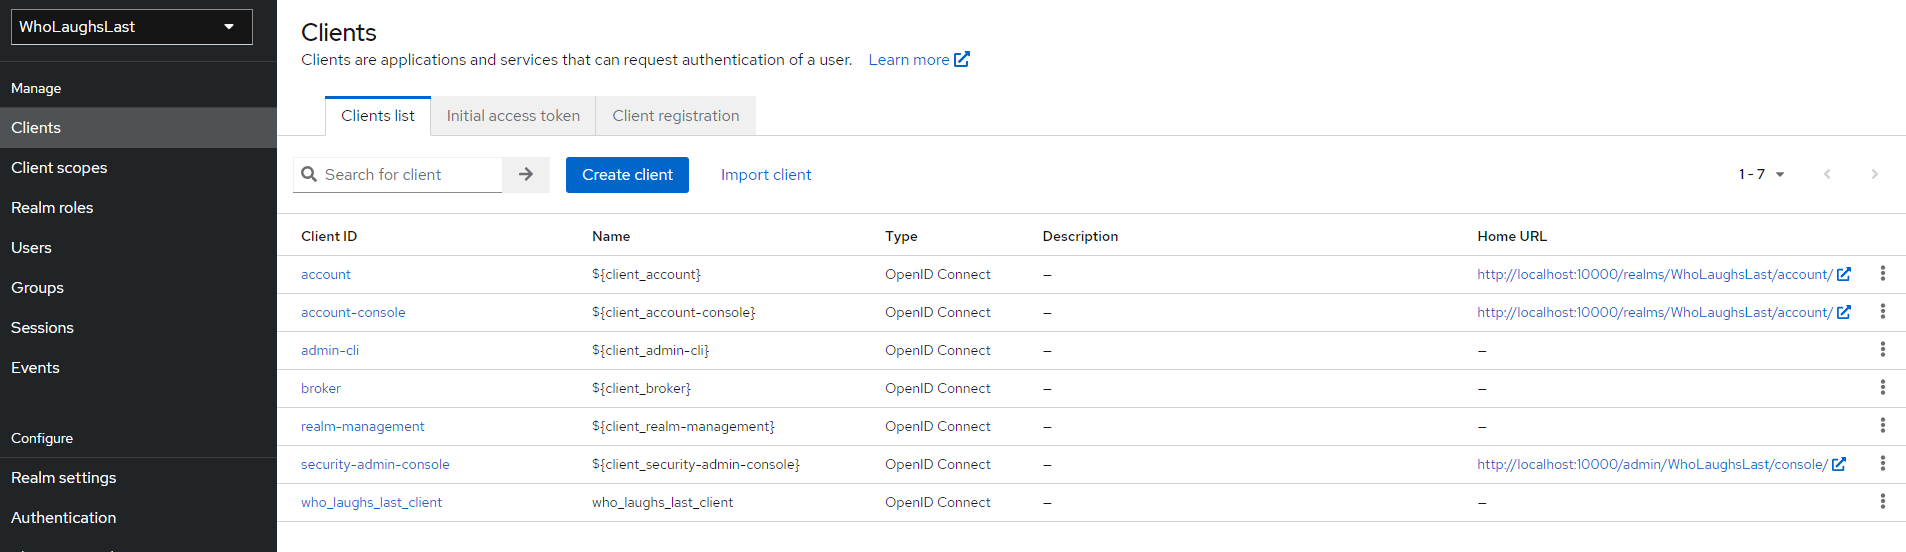
\includegraphics[scale=0.5]{keycloak-cients}
	\label{keycloak}
\end{figure}
\newpage


A végpontok biztonságossá tételéhez a \textbf{Spring Security}-t és az \textbf{OAuth2ResourceServer} dependency-ket használtam fel. A függőségeket leíró xml-eket beillesztettem a pom.xml fájlba, majd a Maven letöltötte őket, hogy majd használni tudjam (\ref{pom}.ábra).
\begin{figure}
	\caption{A pom.xml fileban a függőségek}
	\centering
	\begin{lstlisting}[language=XML]
<dependency>
	<groupId>org.springframework.boot</groupId>
	<artifactId>spring-boot-starter-oauth2-resource-server</artifactId>
	<version>3.1.5</version>
</dependency>
<dependency>
	<groupId>org.springframework.boot</groupId>
	<artifactId>spring-boot-starter-security</artifactId>
	<version>3.1.5</version>
</dependency>
	\end{lstlisting}
	\label{pom}
\end{figure}


Miután a Spring Security bekerül az alkalmazásban, alapértelmezetten csinál egy SecurityFilterChain-t ami megköveteli hogy az összes API végpontnál
a hívónak authetntikálnia kell magát. Ezt a függvényt kell felülírni és úgy implementálni ahogyan azt mi szeretnénk. \textbf{@Bean} annotációval van ellátva,
így ezt a Spring kezeli és tudja hogy mikor kell használni. A kérések beérkeznek az alkalmazásunkba, akkor végighaladnak ezeken a filtereken amiket beállítunk. Miután talál 
egy olyan filtert ami a kéréshez illik: Például a "/board" végződésű végpontra jött kérés, akkor azt tudja hogy authentikálni kell, és a többi filtert már nem nézi meg, akár illik rá akár nem. 

\begin{figure}[h]
	\caption{SecurityFilterChain működése }
	\centering
	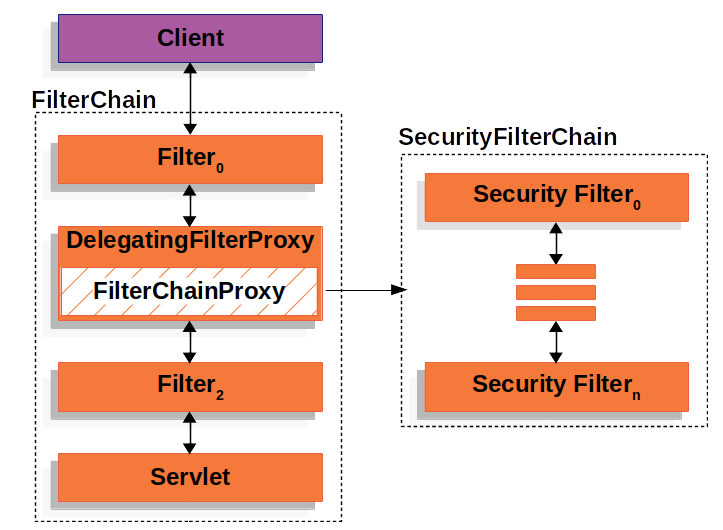
\includegraphics[scale=0.5]{filterchain}
\end{figure}

Úgy konfiguráltam fel a függvényt, hogy 3 végponton kívül mindent authetnikáljon: \textbf{/auth/createToken}, \textbf{/auth/refreshToken} ,\textbf{/subscribe}. Első kettőt végpontot azért nem kell authentikálni, mivel ide érkeznek azok a kérések amikor a felhasználó be akar jelentkezni, és kapja meg a szükséges token-eket amikre majd később szüksége lesz az authentikációnál.Ezek után a OAuth2 resource szervert kellett felkonfigurálni. Az application.yml file-ban írtam bele a különböző elérési utakat amikre a szervernek szüksége van hogy authentikálni tudja a jwt \footnote{Json Web Token} tokeneket. A keycloak-nál a \textbf{http://localhost:10000/realms/WhoLaughsLast/protocol/openid-connect/certs} elérési úton 
elérhető az adott client-hez tartozó authetnikációs adatok. A jwt tokeneket a http kérések fejlécében küldtem el mint BearerTokenek. Hogy ezekhez hozzá tudjak jutni,
egy Convertert kellett írni, majd a OAuth szerver ellenőrizze a hitelességüket. 

\begin{figure}
	\caption{SecurityConfig implementálása}
	\centering
\begin{lstlisting}[language=java]
@Bean
public SecurityFilterChain securityFilterChain (HttpSecurity http) throws Exception{
	http
	.cors().and()
	.csrf()
	.disable()
	.authorizeHttpRequests(authorize -> authorize.
	requestMatchers("/auth/createToken","/subscribe","/auth/refreshToken")
	.permitAll()
	.anyRequest().
	authenticated()).oauth2ResourceServer()
	.jwt().jwtAuthenticationConverter(jwtAuthConverter);
	http
	.sessionManagement()
	.sessionCreationPolicy(STATELESS);
	
	return http.build();
}
\end{lstlisting}
\label{secConf}
\end{figure}
\newpage

Ezek után implementáltam az autentikációs végpontot (\ref{authEndpoint}. ábra). Létrehoztam egy új Controllert aminek AuthController lett a neve,
hogy szeparáltan legyen a többi végponttól ami a játékhoz kell, az átláthatóság és a rendezettség érdekében. Az egyik végpont 
funkciója az hogy egy paraméterben kapott authorization code-ot elküldi a keycloak végpontjára amiért cserébe egy refresh tokent és egy access tokent kap,
és ezeket juttatja el a frontendre. A másik végpont funkciója pedig az hogy egy paraméterben kapott refresh tokent beváltva új access tokent kapjon a frontend az autentikációhoz. 

\begin{figure}[h]
	\caption{Authentikációs végpont}
	\centering
	\begin{lstlisting}[language=java]
		
@PostMapping("/createToken")
public TokenDTO createToken(@RequestBody AuthTokenDTO authCode) throws Exception{
	return authService.getTokens(authCode.getAuthCode());
}		

@PostMapping("/refreshToken")
public TokenDTO refreshAccesToken(@RequestBody RefreshTokenDTO refreshTokenDTO)
throws Exception{
	return authService.refreshAccesTokenWithRefreshToken(refreshTokenDTO
	.getRefresh_token());
}
		
	\end{lstlisting}
	\label{authEndpoint}
\end{figure} 


\begin{figure}[h]
	\caption{Postman authentikációs token kérés}
	\label{fig:postman}
	\centering
	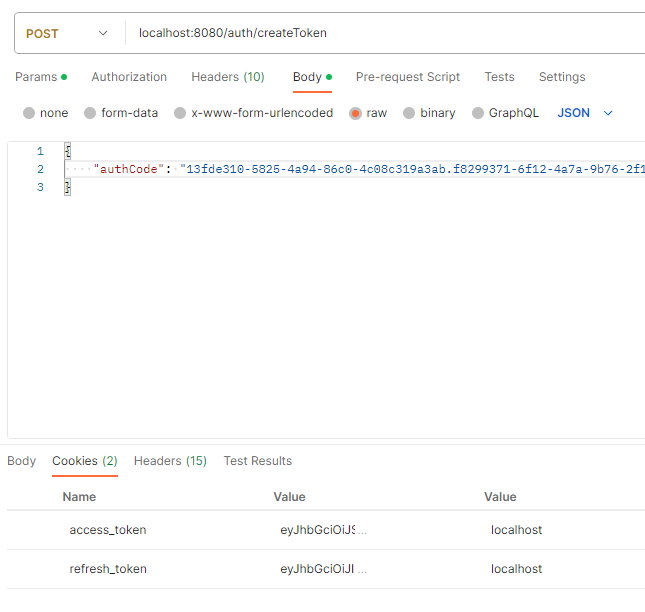
\includegraphics[scale=0.5]{getTokens}
\end{figure}


\subsubsection{Frontend}
A frontenden az autentikáció egyik feladata az authorization code eljuttatása a backend-re volt. Mivel használni akartam a keycloak által 
készített login paget, így az URL-ből kellett kivennem a code-nak az értékét. Mivel a megfelelő bejelentkezés után a keycloak átnavigál a frontend 
URL-jére, hiszen ezt beállítottuk az admin oldalon, így ezt az eseményt fel tudtam használni. Vue Routert használok a navigációra az alkalmazáson belül. A Vue Router 
sok hasznos funkcióval rendelkezik, de ennél a problémánál a navigációs őröket (Navigation Guards) tudtam felhasználni. Itt meg tudok adni egy függvényt ami
mindig meghívódik azelőtt hogy navigáció történne az alkalmazáson belül. Tehát amikor megtörténik a navigáció a keycloak-os felületről az alkalmazásra, a függvény amit 
definiálok le fog futni. Paraméterként megkapom azt az elérési utat ahonnan navigáltak, valamint azt is ahonnan navigáltak. Mivel ahonnan navigálunk el ott jelenik meg az
authorization code, így ki tudom nyerni onnan (\ref{authCode}.ábra). Egy újabb Pinia Store-t is definiáltam az autentikációhoz köthető függvények miatt a jó strukturáltság érdekében. Definiáltam egy \textbf{authTokens} változót is ami az éppen aktuális access és refresh tokeneket tartalmazza. Itt implementáltam egy API hívást, ami http kérés body-jában tárolja az authorization code-ot és küldi el a backend számára. A választ eltárolom az authTokens változóban, így ezekkel már el tudom érni a backenden a játékhoz tartozó védett végpontokat is. 
\begin{figure}
	\caption{Authorization code kinyerése az elnavigált URL-ből}
	\begin{adjustwidth}{0cm}{10cm}
		\begin{minipage}{\textwidth}
			\begin{lstlisting}[style=javascriptStyle]
				router.beforeEach(async (to,from,next) => {
					const authStore = useAuthenticationStore();
					if(to.query.code) {
						await authStore.getAuthTokens({code: to.query.code});
						next(to.path);
					}
					else if(to.name === "playing" && !from.name) {
						next("/boardManagement");
					}
					else {
						next();
					}
					
					
				})
			\end{lstlisting}
		\end{minipage}
	\end{adjustwidth}
	\label{authCode}
\end{figure}

A másik fontos dolog volt implementálni az új access token kérését frontenden. Amint lejárt az addig használt access token érvényessége a szerver 401-es Unauthorized 
hibakóddal tért vissza. Ilyenkor kellett a refresh tokent használni hogy új access tokent kapjunk. Az axios könyvtárat használtam a http kérések küldésére. Az axios 
használatakor létrehozunk egy példányt belőle amik tartalmazzák azokat a függvényeket amikkel a http kéréseket el tudjuk küldeni, például a get,post,delete,stb... Amikor létrehozunk egy ilyen példányt, konfigurálhatjuk úgy, hogy minden egyes kérés küldésekor vagy válasz fogadásánál, bizonyos dolgokat végezzen el. Nekem arra volt szükségem hogy minden kérés elküldésekor a http fejlécébe csatolja az éppen aktuális access tokent, hogy majd a backend autentikálni tudja. Valamint minden egyes beérkezett válasznál ellenőriznem kellett, hogy a válasz 401-es hibakóddal tér-e vissza, mert akkor lejárt az access token, és újat kell kérni. Így ebben a részben hívtam meg az implementált API kérést, majd az újonnan kapott tokent eltároltam a Store-ban, majd ezek után újra elküldtem a meghiúsult API kérést. Mivel egy 
pinia store-ban tároltam el az autentikációs tokeneket, így ha a felhasználó frissíti az oldalt, ezek mind elvesznek. Így erre az eshetőségre is fel kellett konfigurálni az API hívásokat, hogyha nincsenek tokenek, akkor navigáljon el a bejelentkező oldalra. Ilyenkor viszont azt az API hívás amit a frissítés után akarunk végre-hajtani, eldobjuk. Viszont ez nem jelenti azt hogy minden egyes frissítéskor be kell jelentkeznünk, hiszen a Keycloak számon tartja, hogy be vagyunk jelentkezve, ezért rögtön vissza is navigál arra az URL-re amit megadtunk neki (\ref{axios}.ábra).

\begin{figure}
 	\caption{Axios hívások felkonfigurálása autentikáció kezelésére}
 	\begin{adjustwidth}{0cm}{10cm}
 		\begin{minipage}{\textwidth}
 			\begin{lstlisting}[style=javascriptStyle]
 				const AxiosWithToken = axios.create({
 					baseURL: 'http://localhost:8080/'
 				});
 				
 				AxiosWithToken.interceptors.request.use(config => {
 					const authStore = useAuthenticationStore();
 					if(authStore.authTokens){
 						config.headers.Authorization = `Bearer ${authStore.authTokens.access_token}`;
 						return config;
 					}
 					
 				})
 				
 				AxiosWithToken.interceptors.response.use(response =>{
 					return response;
 				},async error=> {
 					const authStore = useAuthenticationStore();
 					if(error.response.status === 401 && authStore.authTokens.refresh_token) {
 						await authStore.getNewAccesTokenWithRefreshToken();
 						return AxiosWithToken(error.config);
 					}
 					else if(!authStore.authTokens.access_token){
 						window.location.href="http://localhost:10000/realms/WhoLaughsLast/protocol/openid-connect/auth?response_type=code&client_id=who_laughs_last_client";
 						return Promise.reject(error.config);
 					}
 				})
 			\end{lstlisting}
 		\end{minipage}
 	\end{adjustwidth}
 	\label{axios}
\end{figure}

\newpage

\subsection{Frontend}
A frontend készítésnél már volt egy kiinduló gitlab projektem, amit a külső konzulensem
biztosított számomra. Ez a projekt egy üres projekt volt, de a Vue.js keretrendszer, webpack
konfiguráció már importálva volt, valamint sok hasznos könyvtárat tartalmazott. Ahogy
korábban említettem, a Vue.js egy komponens orientált fejlesztés tesz lehetővé. Ezt használva
először azt terveztem meg hogy milyen komponensekből fog állni a megjelenítés.
Először a táblák megjelenítéséért felelős komponenst írtam meg. Ez listázza az összes
szerveren lévő táblát.
Következőleg az egy táblát reprezentáló komponenst implementáltam le. Itt látszódnak a tábla
fontosabb adatai, a különböző funkciójú gombok.
A Pinis Store implementálása következett. Itt definiáltam majd valósítottam meg az összes
aszinkron api hívást, hogy kényelmesen, az összes komponensből el tudjam érni őket. Itt
tárolom a táblákat, és egyéb megjelenítést segítő változókat.
Ezek után csináltam felugró ablakokat, ha egy játékost szeretnék egy táblához csatlakoztatni,
vagy egy új táblát szeretnénk létrehozni.
Mivel a backendem hibaüzenetet is adhat, hogyha inkonzisztens adatot küldök el, így annak
megjelenítésével is foglalkoznom kellett. Ha hiba adódik akkor, egy egyszerű piros ablak
jelenik meg az oldal tetején, amiben szerepel a hiba leírása. Ez az ablak 2,5 másodperc
elteltével eltűnik.



\newpage
\begin{thebibliography}{9}
	\bibitem{javaspring}
	Java Spring framework.
	
	\bibitem{vuejs}
	Vuejs framework.
	
	\bibitem{pinia}
	Pinia Store library.
	
	\bibitem{webpack}
	 Webpack is a static module bundler for modern JavaScript applications.
	 
	 \bibitem{axios}
	 Axios library
	 
	 \bibitem{lombok}
	 Lombok library
	 \bibitem{keycloak}
	 Keycloak library
	 \bibitem{konva}
	 Konva library
	 \bibitem{postman}
	 Postman library
	 \bibitem{swagger}
	 Swagger documentation
\end{thebibliography}

\end{document}